\documentclass[main.tex]{subfiles}
\begin{document}

\section{Introduction}

\subsection{Preliminaries}

We will have convention that for a space time vector $x$ in a chosen frame of reference $\bs{x}$ will mean space part of the vector $x$. $x\cdot y$ will mean Minkowsky inner product:
\begin{equation}
x\cdot y = x^0 y^0 - \bs{x}\cdot \bs{y},
\end{equation}

where $\bs{x}\cdot \bs{y}$ is euclidean inner product in $\R^3$. We will also write $x^2 = x\cdot x$ and $\bs{x}^2 = \bs{x}\cdot\bs{x}.$

When a particle of mass $m$ has a $4$-momentum $p$, 
we will denote it's energy by $E_{\bs{p}} = p^0$. 
Note that

\begin{equation}
E_{\bs{p}} = \sqrt{\bs{p}^2 + m^2}.
\end{equation}

\begin{fact}
If $p, q$ are $4$-momentums of particles of mass $m$, then the expression
\begin{equation}
E_{\bs{q}}\delta^{(3)}(\bs{p} - \bs{q})
\end{equation}
is Lorentz invariant. 
\end{fact}
\begin{proof}
Take Lorentz transformation
\begin{equation}
\begin{cases}
E_{\bs{p}'} = p'^0 = \gamma p^0 - \beta\gamma p^1, \\
p'^1 = \gamma p^1 - \beta\gamma E_{\bs{p}}.
\end{cases}
\end{equation}

Let's calculate 
\begin{multline*}
\\
\delta^{(3)}(\bs{p'} - \bs{q'}) = \delta((p'^1 - q'^1, p'^2 - q'^2, p'^3 - q'^3))\\
= \delta((\gamma p^1 - \beta\gamma E_{\bs{p}} - \gamma q^1 + \beta\gamma E_{\bs{q}},p^2 - q^2, p^3 - q^3)).\\
\\
\end{multline*}
Note that
\begin{equation}
\cfrac{\partial}{\partial p^k} E_{\bs{p}} = \cfrac{\partial}{\partial p^k} \sqrt{\bs{p}^2 + m^2} =
\cfrac{p^k}{E_{\bs{p}}}.
\end{equation}

Then 
\begin{multline*}
\\
\cfrac{\partial}{\partial p^1}(\gamma p^1 - \beta\gamma E_{\bs{p}} - \gamma q^1 + \beta\gamma E_{\bs{q}})\\
\\ = \gamma - \cfrac{\beta\gamma p^1}{E_{\bs{q}}} = \cfrac{E_{\bs{p}}\gamma - \beta\gamma p^1}{E_{\bs{p}}} = \cfrac{E_{\bs{p}'}}{E_{\bs{p}}}.
\\ 
\end{multline*}

Let's write Jacobian

\begin{equation}
\bigg|\cfrac{\partial(\bs{p'} - \bs{q'})}{\partial \bs{p}} \bigg|=
\begin{vmatrix}
\cfrac{E_{\bs{p}'}}{E_{\bs{p}}} & \cfrac{\beta\gamma p^2}{E_{\bs{p}}} & \cfrac{\beta\gamma p^3} 
{E_{\bs{p}}} \\
0 & 1 & 0 \\
0 & 0 & 1
\end{vmatrix} = \cfrac{E_{\bs{p}'}}{E_{\bs{p}}}.
\end{equation}

By Theorem \ref{delta-zeros}, we have
\begin{equation}
 \delta(\bs{p}' - \bs{q}') = \bigg(\bigg|\cfrac{\partial(\bs{p'} - \bs{q'})}{\partial \bs{p}} \bigg|_{\bs{p}=\bs{q}}\bigg)^{-1} \delta(\bs{p} - \bs{q}) =
\cfrac{E_{\bs{q}}}{E_{\bs{q}'}} \delta(\bs{p} - \bs{q}).
\end{equation}




Thus
\begin{equation}
E_{\bs{q}'} \delta^{(3)}(\bs{p'} - \bs{q'}) = E_{\bs{q}}\delta^{(3)}(\bs{p} - \bs{q}).
\end{equation}
\end{proof}

\paragraph{Klein-Gordon equation}

For a relativistic particle $E^2 = \bs{p}^2 + m^2$, there is an idea for relativistic  Schrödinger equation
\begin{equation}
i\hbar \cfrac{\partial}{\partial t}\ket{\phi(t)} =  \sqrt{\bs{P}^2 + m^2} \ket{\phi(t)}.
\end{equation}

which is a motivation for a "squared" version (we will set $\hbar=1$):
\begin{equation}
-\cfrac{\partial^2}{\partial t^2} = \bs{P}^2 + m^2,
\end{equation}
which is
\begin{equation}
-\cfrac{\partial^2}{\partial t^2} = -\nabla^2 + m^2,
\end{equation}
or
\begin{equation}
\cfrac{\partial^2}{\partial t^2} - \nabla^2 + m^2 = 0.
\end{equation} 
Can be noted using raised index of partial derivative and Einstein summation convention:
\begin{equation}
\partial^\mu\partial_\mu + m^2 = 0.
\end{equation}
From this immediately follows Lorentz invariance, but we will give a direct proof in language of tensor transformations Figure \ref{klein-proof}.

\begin{figure}
\label{klein-proof}
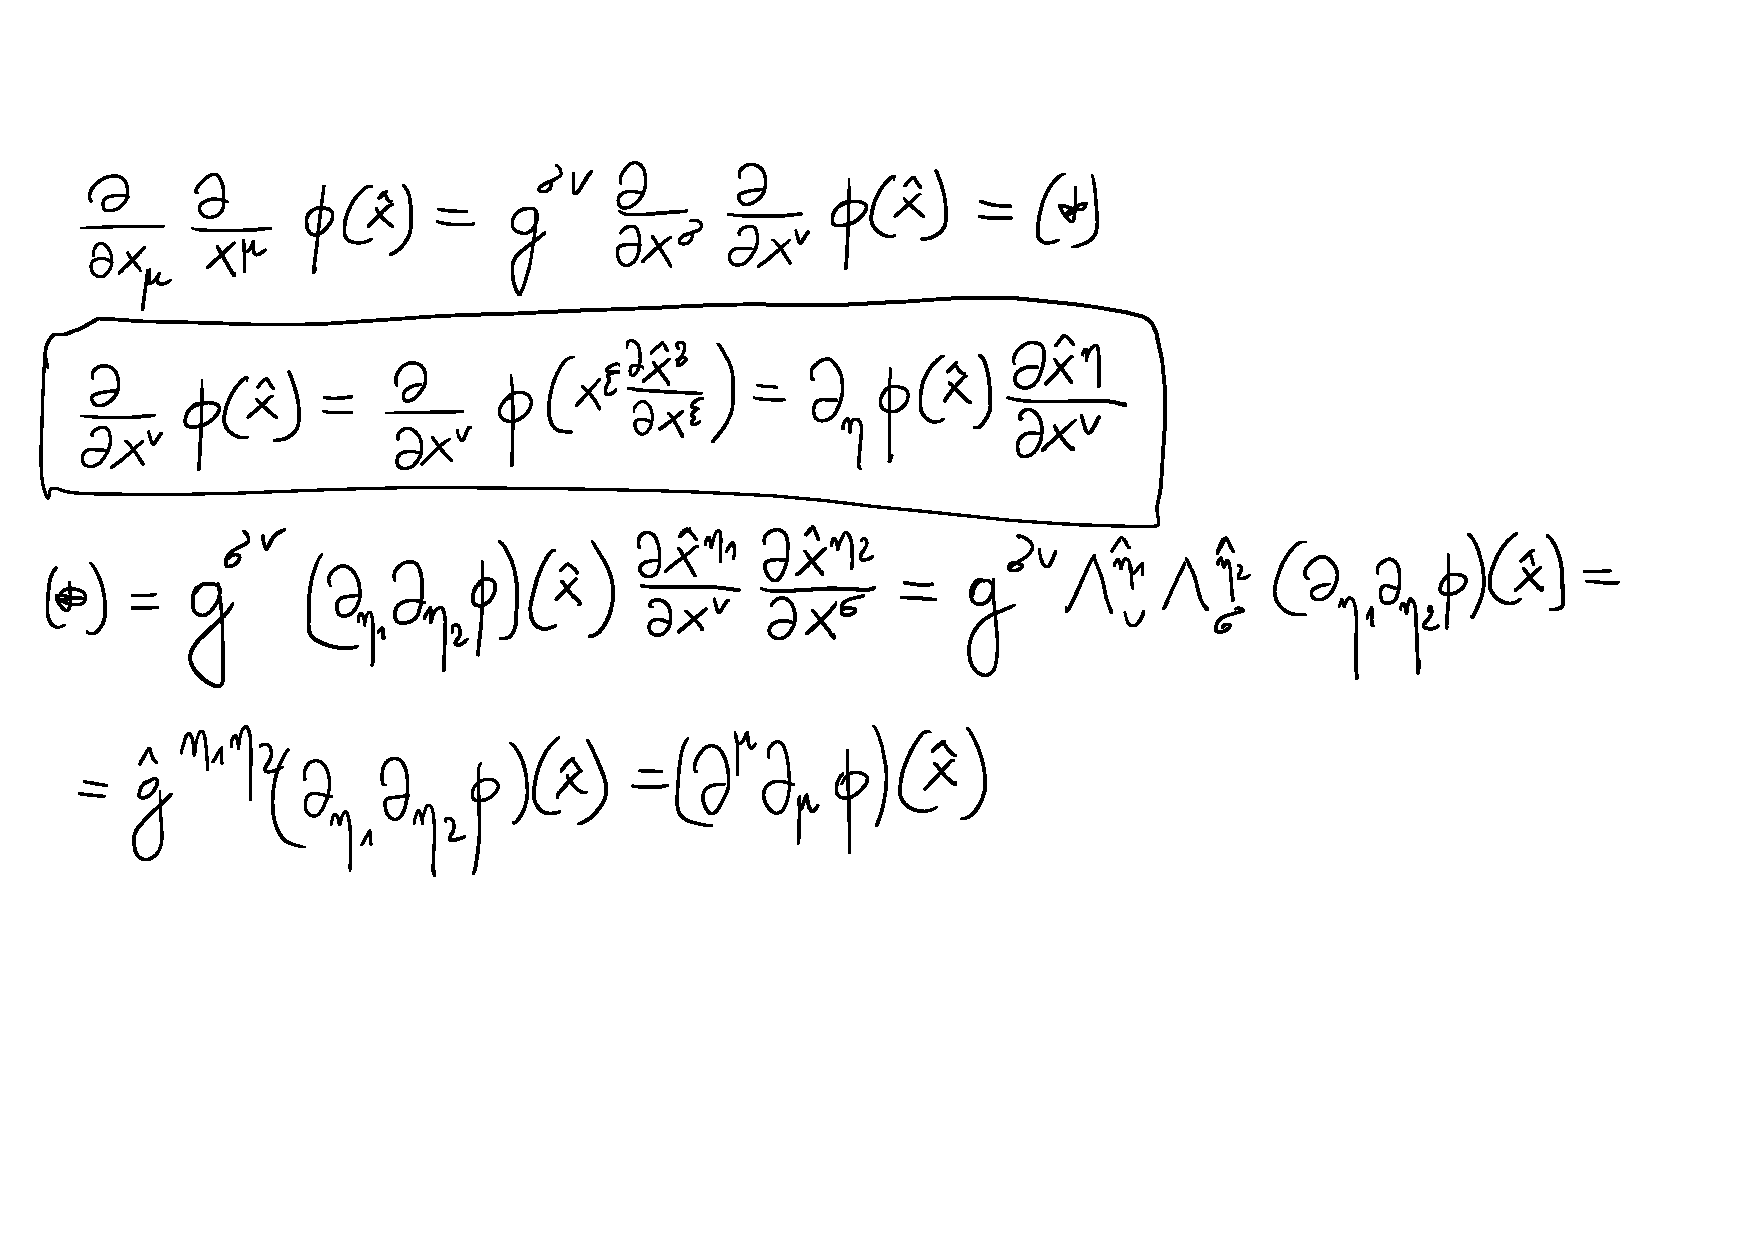
\includegraphics[scale=0.5]{figs/KleinInvariance}
\caption{Proof of Lorentz invariance of Klein-Gordon equation}
\end{figure}
\end{document}